\documentclass[]{article}
\usepackage{lmodern}
\usepackage{amssymb,amsmath}
\usepackage{ifxetex,ifluatex}
\usepackage{fixltx2e} % provides \textsubscript
\ifnum 0\ifxetex 1\fi\ifluatex 1\fi=0 % if pdftex
  \usepackage[T1]{fontenc}
  \usepackage[utf8]{inputenc}
\else % if luatex or xelatex
  \ifxetex
    \usepackage{mathspec}
  \else
    \usepackage{fontspec}
  \fi
  \defaultfontfeatures{Ligatures=TeX,Scale=MatchLowercase}
\fi
% use upquote if available, for straight quotes in verbatim environments
\IfFileExists{upquote.sty}{\usepackage{upquote}}{}
% use microtype if available
\IfFileExists{microtype.sty}{%
\usepackage[]{microtype}
\UseMicrotypeSet[protrusion]{basicmath} % disable protrusion for tt fonts
}{}
\PassOptionsToPackage{hyphens}{url} % url is loaded by hyperref
\usepackage[unicode=true]{hyperref}
\hypersetup{
            pdftitle={Air quality project : Time Series Analysis},
            pdfauthor={Yousra Cherkaoui Tangi - Lou Peltier - Guilhem Bois},
            pdfborder={0 0 0},
            breaklinks=true}
\urlstyle{same}  % don't use monospace font for urls
\usepackage[margin=1in]{geometry}
\usepackage{color}
\usepackage{fancyvrb}
\newcommand{\VerbBar}{|}
\newcommand{\VERB}{\Verb[commandchars=\\\{\}]}
\DefineVerbatimEnvironment{Highlighting}{Verbatim}{commandchars=\\\{\}}
% Add ',fontsize=\small' for more characters per line
\usepackage{framed}
\definecolor{shadecolor}{RGB}{248,248,248}
\newenvironment{Shaded}{\begin{snugshade}}{\end{snugshade}}
\newcommand{\KeywordTok}[1]{\textcolor[rgb]{0.13,0.29,0.53}{\textbf{#1}}}
\newcommand{\DataTypeTok}[1]{\textcolor[rgb]{0.13,0.29,0.53}{#1}}
\newcommand{\DecValTok}[1]{\textcolor[rgb]{0.00,0.00,0.81}{#1}}
\newcommand{\BaseNTok}[1]{\textcolor[rgb]{0.00,0.00,0.81}{#1}}
\newcommand{\FloatTok}[1]{\textcolor[rgb]{0.00,0.00,0.81}{#1}}
\newcommand{\ConstantTok}[1]{\textcolor[rgb]{0.00,0.00,0.00}{#1}}
\newcommand{\CharTok}[1]{\textcolor[rgb]{0.31,0.60,0.02}{#1}}
\newcommand{\SpecialCharTok}[1]{\textcolor[rgb]{0.00,0.00,0.00}{#1}}
\newcommand{\StringTok}[1]{\textcolor[rgb]{0.31,0.60,0.02}{#1}}
\newcommand{\VerbatimStringTok}[1]{\textcolor[rgb]{0.31,0.60,0.02}{#1}}
\newcommand{\SpecialStringTok}[1]{\textcolor[rgb]{0.31,0.60,0.02}{#1}}
\newcommand{\ImportTok}[1]{#1}
\newcommand{\CommentTok}[1]{\textcolor[rgb]{0.56,0.35,0.01}{\textit{#1}}}
\newcommand{\DocumentationTok}[1]{\textcolor[rgb]{0.56,0.35,0.01}{\textbf{\textit{#1}}}}
\newcommand{\AnnotationTok}[1]{\textcolor[rgb]{0.56,0.35,0.01}{\textbf{\textit{#1}}}}
\newcommand{\CommentVarTok}[1]{\textcolor[rgb]{0.56,0.35,0.01}{\textbf{\textit{#1}}}}
\newcommand{\OtherTok}[1]{\textcolor[rgb]{0.56,0.35,0.01}{#1}}
\newcommand{\FunctionTok}[1]{\textcolor[rgb]{0.00,0.00,0.00}{#1}}
\newcommand{\VariableTok}[1]{\textcolor[rgb]{0.00,0.00,0.00}{#1}}
\newcommand{\ControlFlowTok}[1]{\textcolor[rgb]{0.13,0.29,0.53}{\textbf{#1}}}
\newcommand{\OperatorTok}[1]{\textcolor[rgb]{0.81,0.36,0.00}{\textbf{#1}}}
\newcommand{\BuiltInTok}[1]{#1}
\newcommand{\ExtensionTok}[1]{#1}
\newcommand{\PreprocessorTok}[1]{\textcolor[rgb]{0.56,0.35,0.01}{\textit{#1}}}
\newcommand{\AttributeTok}[1]{\textcolor[rgb]{0.77,0.63,0.00}{#1}}
\newcommand{\RegionMarkerTok}[1]{#1}
\newcommand{\InformationTok}[1]{\textcolor[rgb]{0.56,0.35,0.01}{\textbf{\textit{#1}}}}
\newcommand{\WarningTok}[1]{\textcolor[rgb]{0.56,0.35,0.01}{\textbf{\textit{#1}}}}
\newcommand{\AlertTok}[1]{\textcolor[rgb]{0.94,0.16,0.16}{#1}}
\newcommand{\ErrorTok}[1]{\textcolor[rgb]{0.64,0.00,0.00}{\textbf{#1}}}
\newcommand{\NormalTok}[1]{#1}
\usepackage{longtable,booktabs}
% Fix footnotes in tables (requires footnote package)
\IfFileExists{footnote.sty}{\usepackage{footnote}\makesavenoteenv{long table}}{}
\usepackage{graphicx,grffile}
\makeatletter
\def\maxwidth{\ifdim\Gin@nat@width>\linewidth\linewidth\else\Gin@nat@width\fi}
\def\maxheight{\ifdim\Gin@nat@height>\textheight\textheight\else\Gin@nat@height\fi}
\makeatother
% Scale images if necessary, so that they will not overflow the page
% margins by default, and it is still possible to overwrite the defaults
% using explicit options in \includegraphics[width, height, ...]{}
\setkeys{Gin}{width=\maxwidth,height=\maxheight,keepaspectratio}
\IfFileExists{parskip.sty}{%
\usepackage{parskip}
}{% else
\setlength{\parindent}{0pt}
\setlength{\parskip}{6pt plus 2pt minus 1pt}
}
\setlength{\emergencystretch}{3em}  % prevent overfull lines
\providecommand{\tightlist}{%
  \setlength{\itemsep}{0pt}\setlength{\parskip}{0pt}}
\setcounter{secnumdepth}{0}
% Redefines (sub)paragraphs to behave more like sections
\ifx\paragraph\undefined\else
\let\oldparagraph\paragraph
\renewcommand{\paragraph}[1]{\oldparagraph{#1}\mbox{}}
\fi
\ifx\subparagraph\undefined\else
\let\oldsubparagraph\subparagraph
\renewcommand{\subparagraph}[1]{\oldsubparagraph{#1}\mbox{}}
\fi

% set default figure placement to htbp
\makeatletter
\def\fps@figure{htbp}
\makeatother


\title{Air quality project : Time Series Analysis}
\author{Yousra Cherkaoui Tangi - Lou Peltier - Guilhem Bois}
\date{12 janvier, 2020}

\begin{document}
\maketitle

\tableofcontents
\newpage
\section{Preliminary }

Our project consists of time series analysis using R programming
language. Our data set contains the responses of a gas mutisensor device
deployed on the field in an Italian city, in a significantly polluted
area, at road level. The data set contains 9358 instances of hourly
averaged responses from an array of 5 metal oxide chemical sensors
embedded in an Air Quality Chemical Multisensor Device. Data were
recorded from March 2004 to February 2005.

\begin{Shaded}
\begin{Highlighting}[]
\KeywordTok{dim}\NormalTok{(data)}
\end{Highlighting}
\end{Shaded}

\begin{verbatim}
## [1] 9471   17
\end{verbatim}

\begin{Shaded}
\begin{Highlighting}[]
\KeywordTok{str}\NormalTok{(data)}
\end{Highlighting}
\end{Shaded}

\begin{verbatim}
## 'data.frame':    9471 obs. of  17 variables:
##  $ Date         : chr  "10/03/2004" "10/03/2004" "10/03/2004" "10/03/2004" ...
##  $ Time         : chr  "18.00.00" "19.00.00" "20.00.00" "21.00.00" ...
##  $ CO.GT.       : chr  "2,6" "2" "2,2" "2,2" ...
##  $ PT08.S1.CO.  : int  1360 1292 1402 1376 1272 1197 1185 1136 1094 1010 ...
##  $ NMHC.GT.     : int  150 112 88 80 51 38 31 31 24 19 ...
##  $ C6H6.GT.     : chr  "11,9" "9,4" "9,0" "9,2" ...
##  $ PT08.S2.NMHC.: int  1046 955 939 948 836 750 690 672 609 561 ...
##  $ NOx.GT.      : int  166 103 131 172 131 89 62 62 45 -200 ...
##  $ PT08.S3.NOx. : int  1056 1174 1140 1092 1205 1337 1462 1453 1579 1705 ...
##  $ NO2.GT.      : int  113 92 114 122 116 96 77 76 60 -200 ...
##  $ PT08.S4.NO2. : int  1692 1559 1555 1584 1490 1393 1333 1333 1276 1235 ...
##  $ PT08.S5.O3.  : int  1268 972 1074 1203 1110 949 733 730 620 501 ...
##  $ T            : chr  "13,6" "13,3" "11,9" "11,0" ...
##  $ RH           : chr  "48,9" "47,7" "54,0" "60,0" ...
##  $ AH           : chr  "0,7578" "0,7255" "0,7502" "0,7867" ...
##  $ X            : logi  NA NA NA NA NA NA ...
##  $ X.1          : logi  NA NA NA NA NA NA ...
\end{verbatim}

\begin{longtable}[]{@{}cl@{}}
\toprule
\begin{minipage}[b]{0.15\columnwidth}\centering\strut
Attribute\strut
\end{minipage} & \begin{minipage}[b]{0.79\columnwidth}\raggedright\strut
Description\strut
\end{minipage}\tabularnewline
\midrule
\endhead
\begin{minipage}[t]{0.15\columnwidth}\centering\strut
Date\strut
\end{minipage} & \begin{minipage}[t]{0.79\columnwidth}\raggedright\strut
Date (DD/MM/YYYY)\strut
\end{minipage}\tabularnewline
\begin{minipage}[t]{0.15\columnwidth}\centering\strut
Time\strut
\end{minipage} & \begin{minipage}[t]{0.79\columnwidth}\raggedright\strut
Time (HH.MM.SS)\strut
\end{minipage}\tabularnewline
\begin{minipage}[t]{0.15\columnwidth}\centering\strut
CO(GT)\strut
\end{minipage} & \begin{minipage}[t]{0.79\columnwidth}\raggedright\strut
True hourly averaged concentration CO in mg/m\^{}3 (reference
analyzer)\strut
\end{minipage}\tabularnewline
\begin{minipage}[t]{0.15\columnwidth}\centering\strut
PT08.S1(CO)\strut
\end{minipage} & \begin{minipage}[t]{0.79\columnwidth}\raggedright\strut
PT08.S1 (tin oxide) hourly averaged sensor response (nominally CO
targeted)\strut
\end{minipage}\tabularnewline
\begin{minipage}[t]{0.15\columnwidth}\centering\strut
NMHC(GT)\strut
\end{minipage} & \begin{minipage}[t]{0.79\columnwidth}\raggedright\strut
True hourly averaged overall Non Metanic Hydro Carbons concentration in
microg/m\^{}3(reference analyzer\strut
\end{minipage}\tabularnewline
\begin{minipage}[t]{0.15\columnwidth}\centering\strut
C6H6(GT)\strut
\end{minipage} & \begin{minipage}[t]{0.79\columnwidth}\raggedright\strut
True hourly averaged Benzene concentration in microg/m\^{}3 (reference
analyzer)\strut
\end{minipage}\tabularnewline
\begin{minipage}[t]{0.15\columnwidth}\centering\strut
PT08.S2(NMHC)\strut
\end{minipage} & \begin{minipage}[t]{0.79\columnwidth}\raggedright\strut
PT08.S2 (titania) hourly averaged sensor response (nominally NMHC
targeted)\strut
\end{minipage}\tabularnewline
\begin{minipage}[t]{0.15\columnwidth}\centering\strut
NOx(GT)\strut
\end{minipage} & \begin{minipage}[t]{0.79\columnwidth}\raggedright\strut
True hourly averaged NOx concentration in ppb (reference analyzer)\strut
\end{minipage}\tabularnewline
\begin{minipage}[t]{0.15\columnwidth}\centering\strut
PT08.S3(NOx)\strut
\end{minipage} & \begin{minipage}[t]{0.79\columnwidth}\raggedright\strut
PT08.S3 (tungsten oxide) hourly averaged sensor response (nominally NOx
targeted)\strut
\end{minipage}\tabularnewline
\begin{minipage}[t]{0.15\columnwidth}\centering\strut
NO2(GT)\strut
\end{minipage} & \begin{minipage}[t]{0.79\columnwidth}\raggedright\strut
True hourly averaged NO2 concentration in microg/m\^{}3 (reference
analyzer)\strut
\end{minipage}\tabularnewline
\begin{minipage}[t]{0.15\columnwidth}\centering\strut
PT08.S4(NO2)\strut
\end{minipage} & \begin{minipage}[t]{0.79\columnwidth}\raggedright\strut
PT08.S4 (tungsten oxide) hourly averaged sensor response (nominally NO2
targeted)\strut
\end{minipage}\tabularnewline
\begin{minipage}[t]{0.15\columnwidth}\centering\strut
PT08.S5(O3)\strut
\end{minipage} & \begin{minipage}[t]{0.79\columnwidth}\raggedright\strut
PT08.S5 (indium oxide) hourly averaged sensor response (nominally O3
targeted)\strut
\end{minipage}\tabularnewline
\begin{minipage}[t]{0.15\columnwidth}\centering\strut
T\strut
\end{minipage} & \begin{minipage}[t]{0.79\columnwidth}\raggedright\strut
Temperature in °C\strut
\end{minipage}\tabularnewline
\begin{minipage}[t]{0.15\columnwidth}\centering\strut
RH\strut
\end{minipage} & \begin{minipage}[t]{0.79\columnwidth}\raggedright\strut
Relative Humidity (\%)\strut
\end{minipage}\tabularnewline
\begin{minipage}[t]{0.15\columnwidth}\centering\strut
AH\strut
\end{minipage} & \begin{minipage}[t]{0.79\columnwidth}\raggedright\strut
AH Absolute Humidity\strut
\end{minipage}\tabularnewline
\bottomrule
\end{longtable}

\section{I)-Cleaning and preprocessing}\subsection{1) Data cleaning}

As we can see in the str(dim) output, our data contains missing values,
some are directly reported as NA and others have been assigned to -200.
It also contains a certain number of numeric variables that are
characters which makes it not directly exploitable and some numbers have
commas within them. For all these reasons, we had to clean our data set
first so that we can exploit it afterwards.

\begin{verbatim}
## Warning: package 'Amelia' was built under R version 3.5.3
\end{verbatim}

\begin{verbatim}
## Loading required package: Rcpp
\end{verbatim}

\begin{verbatim}
## Warning: package 'Rcpp' was built under R version 3.5.3
\end{verbatim}

\begin{verbatim}
## ## 
## ## Amelia II: Multiple Imputation
## ## (Version 1.7.6, built: 2019-11-24)
## ## Copyright (C) 2005-2020 James Honaker, Gary King and Matthew Blackwell
## ## Refer to http://gking.harvard.edu/amelia/ for more information
## ##
\end{verbatim}

\begin{verbatim}
## Warning: package 'data.table' was built under R version 3.5.3
\end{verbatim}

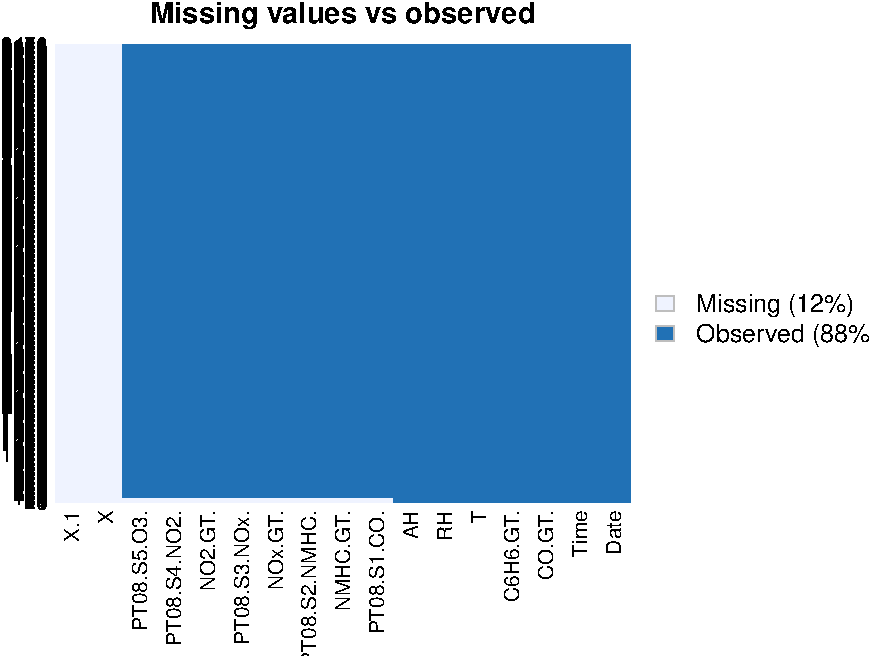
\includegraphics{rapport_files/figure-latex/unnamed-chunk-3-1.pdf}

We remove X1 and X beacause they have no data within them, also we
compute the necessary changes so that our data is exploitable
afterwards.

We noticed that NHMC contains a lot of -200 values, so we prefered to
delet it along with all the lines that contain -200.

\begin{Shaded}
\begin{Highlighting}[]
\KeywordTok{summary}\NormalTok{(data}\OperatorTok{$}\NormalTok{NMHC.GT.)}
\end{Highlighting}
\end{Shaded}

\begin{verbatim}
##    Min. 1st Qu.  Median    Mean 3rd Qu.    Max. 
##  -200.0  -200.0  -200.0  -159.1  -200.0  1189.0
\end{verbatim}

\begin{Shaded}
\begin{Highlighting}[]
\KeywordTok{str}\NormalTok{(data)}
\end{Highlighting}
\end{Shaded}

\begin{verbatim}
## 'data.frame':    6941 obs. of  14 variables:
##  $ Date         : Date, format: "2004-03-10" "2004-03-10" ...
##  $ Time         : chr  "18.00.00" "19.00.00" "20.00.00" "21.00.00" ...
##  $ CO.GT.       : num  2.6 2 2.2 2.2 1.6 1.2 1.2 1 0.9 0.7 ...
##  $ PT08.S1.CO.  : int  1360 1292 1402 1376 1272 1197 1185 1136 1094 1066 ...
##  $ C6H6.GT.     : num  11.9 9.4 9 9.2 6.5 4.7 3.6 3.3 2.3 1.1 ...
##  $ PT08.S2.NMHC.: int  1046 955 939 948 836 750 690 672 609 512 ...
##  $ NOx.GT.      : int  166 103 131 172 131 89 62 62 45 16 ...
##  $ PT08.S3.NOx. : int  1056 1174 1140 1092 1205 1337 1462 1453 1579 1918 ...
##  $ NO2.GT.      : int  113 92 114 122 116 96 77 76 60 28 ...
##  $ PT08.S4.NO2. : int  1692 1559 1555 1584 1490 1393 1333 1333 1276 1182 ...
##  $ PT08.S5.O3.  : int  1268 972 1074 1203 1110 949 733 730 620 422 ...
##  $ T            : num  13.6 13.3 11.9 11 11.2 11.2 11.3 10.7 10.7 11 ...
##  $ RH           : num  48.9 47.7 54 60 59.6 59.2 56.8 60 59.7 56.2 ...
##  $ AH           : num  0.758 0.726 0.75 0.787 0.789 ...
\end{verbatim}

Now that our data is nearly clean, we chose to consider the daily
concentration of the different gases our main focus of study by taking
the average of the concentrations observed daily.

We obtain 341 observations of 13 variables.

\begin{Shaded}
\begin{Highlighting}[]
\KeywordTok{str}\NormalTok{(daily_data)}
\end{Highlighting}
\end{Shaded}

\begin{verbatim}
## 'data.frame':    341 obs. of  13 variables:
##  $ Date         : Date, format: "2004-03-10" "2004-03-11" ...
##  $ CO.GT.       : num  1.97 2.31 2.9 2.74 2.47 ...
##  $ PT08.S1.CO.  : num  1316 1265 1309 1346 1372 ...
##  $ C6H6.GT.     : num  8.45 8.57 12.67 11.38 9.84 ...
##  $ PT08.S2.NMHC.: num  912 880 1036 1010 951 ...
##  $ NOx.GT.      : num  132 150 181 188 150 ...
##  $ PT08.S3.NOx. : num  1167 1233 1053 978 999 ...
##  $ NO2.GT.      : num  109 103 120 120 112 ...
##  $ PT08.S4.NO2. : num  1546 1551 1651 1614 1608 ...
##  $ PT08.S5.O3.  : num  1096 923 1121 1269 1241 ...
##  $ T            : num  12 9.8 11.8 13.4 16.4 ...
##  $ RH           : num  54.9 64.4 49.6 49.9 47.6 ...
##  $ AH           : num  0.766 0.778 0.667 0.734 0.848 ...
\end{verbatim}

\begin{Shaded}
\begin{Highlighting}[]
\KeywordTok{missmap}\NormalTok{(daily_data, }\DataTypeTok{main =} \StringTok{"Missing values vs observed"}\NormalTok{)}
\end{Highlighting}
\end{Shaded}

\includegraphics{rapport_files/figure-latex/unnamed-chunk-10-1.pdf}

Since our data is all observed now, we can start plotting it to
visualize what our data set looks like.

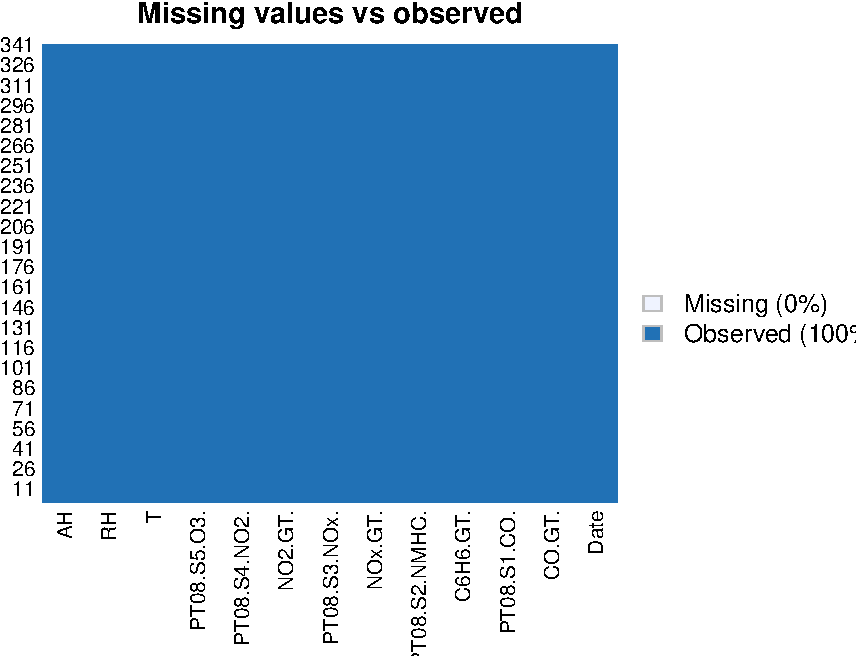
\includegraphics{rapport_files/figure-latex/unnamed-chunk-11-1.pdf}
\includegraphics{rapport_files/figure-latex/unnamed-chunk-11-2.pdf}
\includegraphics{rapport_files/figure-latex/unnamed-chunk-11-3.pdf}

The variables starting with PT are the responses of the sensors
measuring the concentration of the gas concerned. When investigating our
data and by doing some research on air pollution, we found that the main
air pollutants belong to the nitrogen oxides family (NOx). Thus, we
wanted to see the relation between this gas concentration and the other
ones. A linear regression was run between the NOx concentration and the
other gases.

\begin{Shaded}
\begin{Highlighting}[]
\KeywordTok{summary}\NormalTok{(reg)}
\end{Highlighting}
\end{Shaded}

\begin{verbatim}
## 
## Call:
## lm(formula = daily_data$PT08.S3.NOx. ~ +daily_data$PT08.S1.CO. + 
##     daily_data$PT08.S2.NMHC. + daily_data$PT08.S4.NO2. + daily_data$PT08.S5.O3. + 
##     daily_data$T + daily_data$RH + daily_data$AH)
## 
## Residuals:
##     Min      1Q  Median      3Q     Max 
## -182.43  -60.67  -12.99   32.68  736.42 
## 
## Coefficients:
##                            Estimate Std. Error t value Pr(>|t|)    
## (Intercept)              1499.58349   73.78298  20.324  < 2e-16 ***
## daily_data$PT08.S1.CO.     -0.30643    0.09141  -3.352 0.000894 ***
## daily_data$PT08.S2.NMHC.   -0.46111    0.10894  -4.233 2.99e-05 ***
## daily_data$PT08.S4.NO2.     0.51459    0.05633   9.135  < 2e-16 ***
## daily_data$PT08.S5.O3.     -0.26128    0.06138  -4.256 2.70e-05 ***
## daily_data$T               -4.07044    3.05090  -1.334 0.183057    
## daily_data$RH              -0.70990    1.08830  -0.652 0.514660    
## daily_data$AH            -263.09360   48.56193  -5.418 1.16e-07 ***
## ---
## Signif. codes:  0 '***' 0.001 '**' 0.01 '*' 0.05 '.' 0.1 ' ' 1
## 
## Residual standard error: 95.89 on 333 degrees of freedom
## Multiple R-squared:  0.714,  Adjusted R-squared:  0.708 
## F-statistic: 118.8 on 7 and 333 DF,  p-value: < 2.2e-16
\end{verbatim}

We will build the NOx concentration as a time series beacause it comes
from sensor measurements, thus noise will be modeled accordingly. Since
it is linearly related to the other gases (except for the temperature,
relative humidity and absolute humidity that we will exclude from our
study). We will focus on the NOx model.

\subsection{2) Data preprocessing}

We count one PT08.S3.NOX observation per day for 341 days. We suppose
that our time series follows an additive model :

\[
D_t = S_t + T_t +  X_t 
\]

Where \((S_t)_t\) is the seasonality, \((T_t)_t\) the trend and
\((X_t)_t\) is assumed to be stationary.

We obtain this representation :

\includegraphics{rapport_files/figure-latex/unnamed-chunk-14-1.pdf}

Before building any model, we have to stationarise it first by removing
the seasonal and trend components.

\[
X_t = D_t - T_t - S_t
\]

So we use differencing :

\[
D_t - D_{t-1}
\]

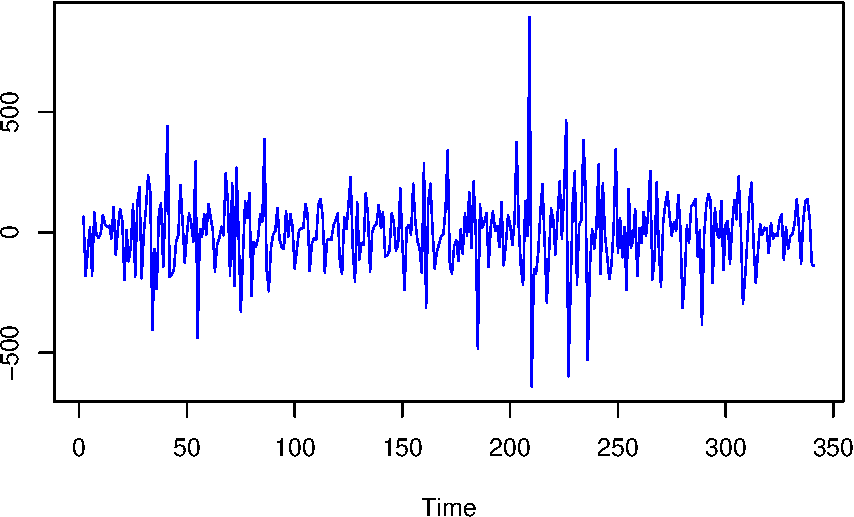
\includegraphics{rapport_files/figure-latex/unnamed-chunk-15-1.pdf}

We want to make sure of the stationarity of our series, so we use the
Augmented Dickey-Fuller Test that tests the null hypothesis that a unit
root is present in a time series sample.

We obtain these results :

\begin{verbatim}
## Warning in adf.test(ts_stat_PT08.S3.NOx.): p-value smaller than printed p-value
\end{verbatim}

\begin{verbatim}
## 
##  Augmented Dickey-Fuller Test
## 
## data:  ts_stat_PT08.S3.NOx.
## Dickey-Fuller = -11.962, Lag order = 6, p-value = 0.01
## alternative hypothesis: stationary
\end{verbatim}

Since our p-value is smalled than 0.01, we reject the null hypothesis
with level of confidence of 99\%

\section{II)-Model fitting on the time series of interest}

In order to test different models, we take out the last 10 most recent
data that will be used for testing, the other observations will be used
for the training.

Let \((X_t)_t\) be a centered second order stationary process. For
\(h \in Z\) , we define :

\begin{itemize}
\tightlist
\item
  The autocovariance function :
\end{itemize}

\[
\gamma_{_X}(h) = Cov(X_t, X_{t+h}) = Cov(X_0, X_h) = E[X_0X_h]
\]

\begin{itemize}
\tightlist
\item
  The autorrelation function (ACF):
\end{itemize}

\[
\rho_{_X}(h) = \rho(X_t, X_{t+h}) = \frac{\gamma_{_X}(h)}{\gamma_{_X}(0)}
\]

\begin{itemize}
\tightlist
\item
  The partial autocorrelation function (PACF):
\end{itemize}

\[
\tilde{\rho}_{_X}(h) = \rho_{_X}(X_0 - \pi_{h-1}(X_0), X_h - \pi_{h-1}(X_h))
\] with the convention \(\pi_0(X_1) = 0\) where \(\pi_{h-1}(X_0)\) is
the projection of \(X_0\) on the linear span of
\((X_1,X_2,....,X_{h-1})\)

\subsection{1) MA model}

A MA(q) process, with \(q \in N\), is a solution to the equation :

\[
X_t = Z_t + \gamma_1Z_{t-1} + ... + \gamma_qZ_{t-q}
\]

with \(t \in Z\) and \((Z_{t})_t\) a white noise.

In order to find q, we use this MA(q) property :

\[
\gamma_{_X}(h) = 0 \ \forall h \ge p
\]

We choose the q parameter accordingly to the last lag in the acf that is
significantly non-null, outside the blue confident band.

\includegraphics{rapport_files/figure-latex/unnamed-chunk-18-1.pdf}

We notice that we can not fit our data into a MA model, which is quite
unexpected, because the data comes from sensor measurements so we have
expected a strong noise presence. Thus, we will try other models.

\subsection{2) AR model}

A second model is the AR(p).

An AR(p) process, with \(p \in N\), is a solution of the equation :

\[
X_t = \phi_{1}X_{t-1} + \phi_{2}X_{t-2} + ... + \phi_{p}X_{t-p} + Z_{t} 
\]

We will use a pacf AR(p) proprety, equivalent to the acf MA(q) property
:

\[
\tilde{\rho}_{_X}(h) = 0 \ \forall h>p 
\] We obtain this pacf plot :

\includegraphics{rapport_files/figure-latex/unnamed-chunk-19-1.pdf}

The PACF plot indicates a significant value at lag 5. Thus, we choose an
AR(5) model.

\begin{verbatim}
## 
## Call:
## arima(x = ts_stat_PT08.S3.NOx._train_set, order = c(5, 0, 0), include.mean = FALSE)
## 
## Coefficients:
##           ar1      ar2      ar3      ar4      ar5
##       -0.2842  -0.3523  -0.3167  -0.2801  -0.1998
## s.e.   0.0539   0.0541   0.0546   0.0538   0.0539
## 
## sigma^2 estimated as 20679:  log likelihood = -2108.17,  aic = 4228.34
\end{verbatim}

So we have :

\[
X_t = -0.2842X_{t-1}-0.3523X_{t-2}-0.3167X_{t-3}-0.2801X_{t-4}-0.1998X_{t-5}
\]

Now we check that the residuals are likely white noise.

\includegraphics{rapport_files/figure-latex/unnamed-chunk-21-1.pdf}

The ACF plot of residuals show no significant lags, so the AR(5) is
likely a good representation of the series. Also, the p-values for
Ljung-Box statistic are all greater than 0.05, so we cannot reject the
hypothesis that the autocorrelation is different from 0. Therefore, the
AR(5) model is an appropriate one.

\subsection{3) ARMA model}

Then, we're going to fit an ARMA model. An ARMA(p,q) time series is a
process solution of the following model :

\[
X_t= \phi_{1}X_{t-1} + \phi_{2}X_{t-2} + ... + \phi_{p}X_{t-p} + Z_{t} + \gamma_1Z_{t-1} + ... + \gamma_qZ_{t-q}
\]

with \[\theta=(\phi_{1},...,\phi_{p},\gamma_1,...,\gamma_q)'\] the
parameters of the model and \(Z_t\) a white noise.

We want to find the ARMA's orders p and q, so we need to use some
information criterion. An information criterion is an estimator of the
relative quality of statistical models for a given set of data. Indeed,
given a collection of models for the data, the information criterion
estimates the quality of each model relative to each of the other
models. So, we will use the results of the AIC to dertermine the orders
of our ARMA model.

The AIC (Akaike Information Criterion) offers an estimate of the
relative information lost when a given model is used to represent the
process that generated the data. So the model with the minimum AIC is
considered as the best model for the given data.

To observe the AIC values obtained we create a matrix with all AIC for
p,q\textless{}6.

\begin{verbatim}
## Warning in arima(ts_stat_PT08.S3.NOx._train_set, order = c(i, 0, j),
## include.mean = FALSE): possible convergence problem: optim gave code = 1
\end{verbatim}

\begin{verbatim}
##          MA1      MA2      MA3      MA4      MA5
## AR1 4211.483 4206.408 4207.209 4208.772 4210.647
## AR2 4204.466 4205.355 4206.963 4208.054 4199.441
## AR3 4205.208 4207.144 4205.511 4210.136 4210.828
## AR4 4206.998 4208.875 4209.925 4206.424 4208.000
## AR5 4208.125 4210.959 4206.094 4213.566 4200.193
\end{verbatim}

We can see that the minimum of AIC is obtained for the ARMA(2,5) model,
so the best model based on the AIC is an ARMA(2,5).

We can now fit our ARMA(2,5) model.

\begin{verbatim}
## Warning in arima(ts_stat_PT08.S3.NOx._train_set, order = c(2, 0, 5),
## include.mean = FALSE): possible convergence problem: optim gave code = 1
\end{verbatim}

\begin{verbatim}
## 
## Call:
## arima(x = ts_stat_PT08.S3.NOx._train_set, order = c(2, 0, 5), include.mean = FALSE)
## 
## Coefficients:
##          ar1      ar2      ma1     ma2      ma3      ma4      ma5
##       1.1177  -0.9836  -1.5211  1.1052  -0.1684  -0.2120  -0.1372
## s.e.  0.0127   0.0122   0.0565  0.1028   0.1191   0.1014   0.0555
## 
## sigma^2 estimated as 18398:  log likelihood = -2091.72,  aic = 4199.44
\end{verbatim}

We have

\[
X_t= 1.1177X_{t-1} - 0.9836X_{t-2} + Z_{t} - 1.5211Z_{t-1} - 1.1052Z_{t-2} - 0.1684Z_{t-3} - 0.2120Z_{t-4} - 0.1372Z_{t-5}
\]

Our model is now fitted so we have to check if the residuals are likely
white noise.

\includegraphics{rapport_files/figure-latex/unnamed-chunk-24-1.pdf}

By looking at the ACF plot of residuals we can notice there is not
significant lag outside the blue confident band which means that the
selected model ARMA(5,5) is a good model to represent the serie.
Moreover, the p-values of the Ljung-Box statistic test are all much
greater than 5\%, so we can't reject the null hypothesis of the
autocorrelation different from 0. The ARMA(5,5) model is an appropriate
model for our time series.

\subsection{4) Residuals}

We have fitted two models, and then e have to choose between these two
models. In order to make this choice, we will look at two information
criterions : the AIC previously used and the BIC a cirterion similar to
the AIC but with a different penalty for the numbers of parameters.

\begin{verbatim}
##                df      AIC
## fit_ar_model    6 4228.336
## fit_arma_model  8 4199.441
\end{verbatim}

\begin{verbatim}
##                df      BIC
## fit_ar_model    6 4251.131
## fit_arma_model  8 4229.833
\end{verbatim}

The smallest AIC and the smallest BIC are bith given for the ARMA(5,5)
model, so we are going to choose this one for the rest of the project.

We want to check the normality of the residuals. We begin our analysis
by plotting the residuals and the suqarred residuals :

\includegraphics{rapport_files/figure-latex/unnamed-chunk-26-1.pdf}

We notice an outlier at time 208 which means something unusual has may
happened this day.

Then we plot the ACF graphs :

\includegraphics{rapport_files/figure-latex/unnamed-chunk-27-1.pdf}

These plots show us there is no autocorrelation remaining in the
residuals which means that the chosen model captures the pattern in the
data effectively.

finally we plot the QQ plot of the residuals to observe their behavior :

\includegraphics{rapport_files/figure-latex/unnamed-chunk-28-1.pdf}

By looking at this graph we can conlude that the residuals don't seem
gaussian as there are too many extreme values, and thus fat tail. The
relationship between sample quantiles and theoretical quantiles is not
linear.

We can validate our hypothesis of the non normality of the residuals by
performing a Jarque-Bera test. This test verify whether sample data have
the skewness and kurtosis corresponding to a normal distribution.

\begin{verbatim}
## 
##  Jarque Bera Test
## 
## data:  eps
## X-squared = 845.98, df = 2, p-value < 2.2e-16
\end{verbatim}

The p-value is smaller than 5\% so we can reject the null hypothesis of
the data normally distributed.

So we can reasonably conclude that the residuals are not gaussians and
so the condition of the normal distribution of the error terms is not
met.

\subsection{5) GARCH model}

We want to fit a GARCH model on the data as an ARMA model is a method to
linerarly model the data. But if we want to model volatility we should
use a GARCH model.

\begin{verbatim}
## Loading required package: timeDate
\end{verbatim}

\begin{verbatim}
## Loading required package: timeSeries
\end{verbatim}

\begin{verbatim}
## Loading required package: fBasics
\end{verbatim}

\begin{verbatim}
## Loading required package: zoo
\end{verbatim}

\begin{verbatim}
## 
## Attaching package: 'zoo'
\end{verbatim}

\begin{verbatim}
## The following object is masked from 'package:timeSeries':
## 
##     time<-
\end{verbatim}

\begin{verbatim}
## The following objects are masked from 'package:base':
## 
##     as.Date, as.Date.numeric
\end{verbatim}

\begin{verbatim}
## 
## Attaching package: 'xts'
\end{verbatim}

\begin{verbatim}
## The following objects are masked from 'package:data.table':
## 
##     first, last
\end{verbatim}

\begin{verbatim}
## Warning: package 'astsa' was built under R version 3.5.3
\end{verbatim}

\begin{verbatim}
## 
## Attaching package: 'astsa'
\end{verbatim}

\begin{verbatim}
## The following object is masked from 'package:fBasics':
## 
##     nyse
\end{verbatim}

The GARCH(p,q) model is the solution (if it exists) to the following
system :

\[
Z_t=\sigma_t W_t \\
\sigma_t^2 = w +\beta_1 \sigma_{t-1}^2 + ... + \beta_p \sigma_{t-p}^2 + \alpha_1 Z_{t-1}^2 +...+ \alpha_p Z_{t-p}^2
\] where (Zt) is an observed white noise.

For simplicity, we focus on a GARCH(1,1) model :

\[
\sigma_t^2 = w +\beta_1 \sigma_{t-1}^2 + \alpha_1 Z_{t-1}^2
\] We fit a GARCH(1,1) model with several functions studied in class. We
obtain this model :

\[
\sigma_t^2 = 1.3679 +0.9383 \sigma_{t-1}^2 + 0.0721 Z_{t-1}^2
\] Then we can check the nullity of \(\beta\) :

\begin{verbatim}
## p-value : 0
\end{verbatim}

The p-value is smaller than 0.05 so we can reject the null hypothesis
(which is \(\beta=0\)). Therefore \(\beta \neq 0\).

We also want to check the nullity of \(\alpha\) :

\begin{verbatim}
## p-value : 0
\end{verbatim}

The p-value is smaller than 0.05 so we can reject the null hypothesis.
Therefore \(\alpha \neq 0\).

\includegraphics{rapport_files/figure-latex/unnamed-chunk-34-1.pdf}

\includegraphics{rapport_files/figure-latex/unnamed-chunk-35-1.pdf} The
GARCH(1,1) residuals don't seem to be gaussian but the ACF graph
obtained shows no autocorrelation remaining in the residuals.

\subsection{6) Prediction intervals for the 10 most recent data}

We want to construct a one-step interval using the rugarch package. We
create a matrix to stock the values of the interval's bounds :

\begin{verbatim}
## Loading required package: parallel
\end{verbatim}

\begin{verbatim}
## 
## Attaching package: 'rugarch'
\end{verbatim}

\begin{verbatim}
## The following object is masked from 'package:stats':
## 
##     sigma
\end{verbatim}

\begin{verbatim}
##       Lower bound Upper bound
##  [1,]   -178.9923    306.5658
##  [2,]   -209.8591    279.2671
##  [3,]   -227.3783    265.1407
##  [4,]   -237.6006    258.1457
##  [5,]   -243.8198    254.9977
##  [6,]   -247.8298    253.9112
##  [7,]   -250.6081    253.9168
##  [8,]   -252.6882    254.4883
##  [9,]   -254.3618    255.3412
## [10,]   -255.7889    256.3218
\end{verbatim}

We can observe our prediction interval on a graph with the previous
values (dark line) and the real values observed (red points) :

\begin{verbatim}
## Warning: package 'ggplot2' was built under R version 3.5.3
\end{verbatim}

\begin{verbatim}
## Warning: Removed 10 rows containing missing values (geom_path).

## Warning: Removed 10 rows containing missing values (geom_path).

## Warning: Removed 10 rows containing missing values (geom_path).
\end{verbatim}

\begin{verbatim}
## Warning: Removed 10 rows containing missing values (geom_point).
\end{verbatim}

\includegraphics{rapport_files/figure-latex/unnamed-chunk-39-1.pdf} We
can notice that the real values are inside our forecast interval,
howerver our interval is not really accurate as it is almost constant
and very large.

\section{III)-Training on the times series of interest using explanatory times series}

Yet, we will introduce other components, that we didn'tuse in the models
previously. We do it in order to find better predictions and better
confidence intervals.

\subsection{1) Preprocessing}

first, we have to stationarise our data with the same method as before.
This means that we remove seasonal and trend components by using
differencing.

\begin{Shaded}
\begin{Highlighting}[]
\KeywordTok{library}\NormalTok{(data.table)}
\CommentTok{#On choisit le fichier qui contient les données}
\NormalTok{path =}\StringTok{ "C:/Users/pelti/OneDrive/Documents/GitHub/Air-Quality-Project/src/cleaningData_bis.R"}
\KeywordTok{source}\NormalTok{(path)}
\end{Highlighting}
\end{Shaded}

\begin{Shaded}
\begin{Highlighting}[]
\KeywordTok{library}\NormalTok{(KFAS)}
\end{Highlighting}
\end{Shaded}

\begin{verbatim}
## Warning: package 'KFAS' was built under R version 3.5.3
\end{verbatim}

\begin{Shaded}
\begin{Highlighting}[]
\KeywordTok{library}\NormalTok{(ggplot2)}
\KeywordTok{ggplot}\NormalTok{(daily_data,  }\KeywordTok{aes}\NormalTok{(}\DataTypeTok{x=}\NormalTok{Date, }\DataTypeTok{y=}\NormalTok{PT08.S4.NO2.)) }\OperatorTok{+}\StringTok{ }\KeywordTok{geom_line}\NormalTok{()}
\end{Highlighting}
\end{Shaded}

\includegraphics{rapport_files/figure-latex/unnamed-chunk-41-1.pdf}

We see indeed that this data need to be stationarised

\begin{Shaded}
\begin{Highlighting}[]
\CommentTok{#we stationarise the dataset}
\NormalTok{ts_PT08.S4.NO2. =}\StringTok{ }\KeywordTok{ts}\NormalTok{(daily_data}\OperatorTok{$}\NormalTok{PT08.S4.NO2., }\DataTypeTok{start=}\DecValTok{1}\NormalTok{, }\DataTypeTok{frequency =}\DecValTok{1}\NormalTok{)}
\NormalTok{ts_stat_PT08.S4.NO2. =}\StringTok{ }\KeywordTok{diff}\NormalTok{(ts_PT08.S4.NO2.)}
\NormalTok{daily_data}\OperatorTok{$}\NormalTok{PT08.S4.NO2._stat <-}\StringTok{ }\KeywordTok{c}\NormalTok{(}\DecValTok{0}\NormalTok{,}\KeywordTok{diff}\NormalTok{(daily_data}\OperatorTok{$}\NormalTok{PT08.S4.NO2.))}
\KeywordTok{ggplot}\NormalTok{(}\DataTypeTok{data=}\NormalTok{daily_data, }\KeywordTok{aes}\NormalTok{(}\DataTypeTok{x=}\NormalTok{Date, }\DataTypeTok{y=}\NormalTok{PT08.S4.NO2._stat)) }\OperatorTok{+}\StringTok{ }\KeywordTok{geom_line}\NormalTok{()}
\end{Highlighting}
\end{Shaded}

\includegraphics{rapport_files/figure-latex/unnamed-chunk-42-1.pdf}

As before, we apply the Augmented Dickey-Fuller Test

\begin{Shaded}
\begin{Highlighting}[]
\KeywordTok{library}\NormalTok{(tseries)}
\NormalTok{test_stationnarity =}\StringTok{ }\KeywordTok{adf.test}\NormalTok{(ts_stat_PT08.S4.NO2.)}
\end{Highlighting}
\end{Shaded}

\begin{verbatim}
## Warning in adf.test(ts_stat_PT08.S4.NO2.): p-value smaller than printed p-value
\end{verbatim}

\begin{Shaded}
\begin{Highlighting}[]
\KeywordTok{print}\NormalTok{(test_stationnarity)}
\end{Highlighting}
\end{Shaded}

\begin{verbatim}
## 
##  Augmented Dickey-Fuller Test
## 
## data:  ts_stat_PT08.S4.NO2.
## Dickey-Fuller = -11.191, Lag order = 6, p-value = 0.01
## alternative hypothesis: stationary
\end{verbatim}

We do it for each component with a name starting with PT.

To be sure that everything is fine, we use the Augmented Dickey-Fuller
Test.

Here are the results of this tests after the stationarisation for each
component.

\includegraphics{rapport_files/figure-latex/unnamed-chunk-44-1.pdf}

\includegraphics{rapport_files/figure-latex/unnamed-chunk-45-1.pdf}

\begin{Shaded}
\begin{Highlighting}[]
\KeywordTok{library}\NormalTok{(tseries)}
\NormalTok{test_stationnarity =}\StringTok{ }\KeywordTok{adf.test}\NormalTok{(ts_stat_PT08.S1.CO.)}
\end{Highlighting}
\end{Shaded}

\begin{verbatim}
## Warning in adf.test(ts_stat_PT08.S1.CO.): p-value smaller than printed p-value
\end{verbatim}

\begin{Shaded}
\begin{Highlighting}[]
\KeywordTok{print}\NormalTok{(test_stationnarity)}
\end{Highlighting}
\end{Shaded}

\begin{verbatim}
## 
##  Augmented Dickey-Fuller Test
## 
## data:  ts_stat_PT08.S1.CO.
## Dickey-Fuller = -11.123, Lag order = 6, p-value = 0.01
## alternative hypothesis: stationary
\end{verbatim}

\includegraphics{rapport_files/figure-latex/unnamed-chunk-47-1.pdf}

\begin{Shaded}
\begin{Highlighting}[]
\CommentTok{#}
\KeywordTok{library}\NormalTok{(tseries)}
\NormalTok{test_stationnarity =}\StringTok{ }\KeywordTok{adf.test}\NormalTok{(ts_stat_PT08.S2.NMHC.)}
\end{Highlighting}
\end{Shaded}

\begin{verbatim}
## Warning in adf.test(ts_stat_PT08.S2.NMHC.): p-value smaller than printed p-value
\end{verbatim}

\begin{Shaded}
\begin{Highlighting}[]
\KeywordTok{print}\NormalTok{(test_stationnarity)}
\end{Highlighting}
\end{Shaded}

\begin{verbatim}
## 
##  Augmented Dickey-Fuller Test
## 
## data:  ts_stat_PT08.S2.NMHC.
## Dickey-Fuller = -11.266, Lag order = 6, p-value = 0.01
## alternative hypothesis: stationary
\end{verbatim}

\includegraphics{rapport_files/figure-latex/unnamed-chunk-49-1.pdf}

\begin{Shaded}
\begin{Highlighting}[]
\CommentTok{#}
\KeywordTok{library}\NormalTok{(tseries)}
\NormalTok{test_stationnarity =}\StringTok{ }\KeywordTok{adf.test}\NormalTok{(ts_stat_PT08.S5.O3.)}
\end{Highlighting}
\end{Shaded}

\begin{verbatim}
## Warning in adf.test(ts_stat_PT08.S5.O3.): p-value smaller than printed p-value
\end{verbatim}

\begin{Shaded}
\begin{Highlighting}[]
\KeywordTok{print}\NormalTok{(test_stationnarity)}
\end{Highlighting}
\end{Shaded}

\begin{verbatim}
## 
##  Augmented Dickey-Fuller Test
## 
## data:  ts_stat_PT08.S5.O3.
## Dickey-Fuller = -11.178, Lag order = 6, p-value = 0.01
## alternative hypothesis: stationary
\end{verbatim}

\subsection{2) Time varying coefficients}

Now we want to build a dynamical model thanks to the explanatory time
series. We know that the order of the AR model was 5, so we will use 5
past values of the time series of interest for predicting the present
value of the time series of interest too.

\begin{verbatim}
##          ytraining lag(ytraining, 1) lag(ytraining, 2) lag(ytraining, 3)
## [334,]  -14.251812         -6.708333          38.74275         138.21558
## [335,]   -6.708333         38.742754         138.21558          22.08333
## [336,]   38.742754        138.215580          22.08333        -131.90761
## [337,]  138.215580         22.083333        -131.90761                NA
## [338,]   22.083333       -131.907609                NA                NA
## [339,] -131.907609                NA                NA                NA
##        lag(ytraining, 4) lag(ytraining, 5) lag(ytraining, 6) lag(ytraining, 7)
## [334,]          22.08333         -131.9076                NA                NA
## [335,]        -131.90761                NA                NA                NA
## [336,]                NA                NA                NA                NA
## [337,]                NA                NA                NA                NA
## [338,]                NA                NA                NA                NA
## [339,]                NA                NA                NA                NA
##        lag(ytraining, 8) lag(ytraining, 9) lag(ytraining, 10)
## [334,]                NA                NA                 NA
## [335,]                NA                NA                 NA
## [336,]                NA                NA                 NA
## [337,]                NA                NA                 NA
## [338,]                NA                NA                 NA
## [339,]                NA                NA                 NA
\end{verbatim}

We use the SSModel function. Our target variable is ts\_PTO8.S3.NOx. and
our covariates are the other components starting with PT.

\begin{verbatim}
## [1] "data.frame"
\end{verbatim}

\subsection{3) QLIK}

We have our model so we can use it with a QFAS in order to tune the
hyperparameter.

\begin{verbatim}
## , , 1
## 
##      [,1] [,2] [,3] [,4]
## [1,]    1    0    0    0
## [2,]    0    1    0    0
## [3,]    0    0    1    0
## [4,]    0    0    0    1
\end{verbatim}

\begin{verbatim}
## , , 1
## 
##      [,1]
## [1,]    1
\end{verbatim}

\includegraphics{rapport_files/figure-latex/unnamed-chunk-53-1.pdf}

We have the covariance matrix of disturbance terms that is the identity.
So we have for each component this result :

\begin{Shaded}
\begin{Highlighting}[]
\CommentTok{# the parameters for the 1 step prediction}
\KeywordTok{plot.ts}\NormalTok{(kal}\OperatorTok{$}\NormalTok{a[,}\DecValTok{1}\OperatorTok{:}\DecValTok{4}\NormalTok{] )}
\end{Highlighting}
\end{Shaded}

\includegraphics{rapport_files/figure-latex/unnamed-chunk-54-1.pdf}

and we find the variance

\begin{Shaded}
\begin{Highlighting}[]
\CommentTok{# the variances estimation as mean square errors for 10 lags}
\NormalTok{sigma <-}\StringTok{ }\KeywordTok{colMeans}\NormalTok{((kal}\OperatorTok{$}\NormalTok{m}\OperatorTok{-}\NormalTok{Y[(n}\OperatorTok{-}\DecValTok{5}\NormalTok{)}\OperatorTok{:}\NormalTok{(n}\OperatorTok{-}\DecValTok{1}\NormalTok{),}\DecValTok{1}\NormalTok{])}\OperatorTok{^}\DecValTok{2}\NormalTok{,}\DataTypeTok{na.rm =} \OtherTok{TRUE}\NormalTok{)   }\CommentTok{# remove a burn-in period to estimate the variances}
\KeywordTok{plot}\NormalTok{(sigma)}
\end{Highlighting}
\end{Shaded}

\includegraphics{rapport_files/figure-latex/unnamed-chunk-55-1.pdf} It
seems that Variances can be seen as constant through time here.

\subsection{4) Prediction}

We have everything yet in order to do the prediction. The intervals of
prediction can indeed be produced thanks to the use of the Kalman's
recursion on the tuned dynamical model.

Let's explain why we use this : by contrast with the AR models, it is
much more difficult to find the best possible (linear) prediction of an
ARMA mode. Indeed, as soon as the MA part is non degenerate, the filter
can have infinitely many non null coefficients.

One way to solve the problem is to consider ARMA model as a more general
linear model called state space models. Those models have been
introduced in signal processing and the best linear prediction can be
computed recursively by the Kalman's recursion. How does this work ? A
state space linear model of dimension r with constant coefficient is
given by a system of space euqation and state equations of the form :
\(X_t = G^TY_t +Z_T\) \(Y_t = FY_{t-1} +V_t\) which are respectively the
Space equation and the State equation, where \((Z_t)\) and \((V_t)\) are
uncorrelated white noise with variance R and Q, G \(\in\) Rr, F \(\in\)
M(r,r) and Y \(\in\) Rr is the random state of the system. The Kalman
theorem says : In a state-space model with constant coefficients, if

\(\widehat{Y_0}\) and \(\Omega_0\) are well chosen, one can compute
recursively

\[ 
\widehat{X_n} = \pi_{n-1}(X_n)
\]

\[\\ R_n^L = E[(X_n - \widehat{X_n})^2] \]

\[\\ \widehat{Y_n} = \pi_{n-1}(Y_n) \]

\[\\and\ \Omega_n = E[(Y_n - \widehat{Y_n})(Y_n - \widehat{Y_n})^T] \]

\[\\by\ the\ following\ recursion\ : \\
\widehat{Y_{n+1}} = F\widehat{Y_n} + \frac{F\Omega_nG}{R_n^L}*(X_n -G^T\widehat{Y_n}) \\\]

\[\widehat{X_{n+1}} = (G)^T*\widehat{Y_{n+1}} \\\]

\[\Omega_{n+1} = F\Omega_nF^T +Q- \frac{F\Omega_nG}{R_n}*G^T\Omega_nF^T \\\]

\[
R_{n+1}^L = G^T\Omega_{n+1}G+R 
\]

Our target variable is ts\_PTO8.S3.NOx. and our covariates are the other
components starting with PT.

\begin{Shaded}
\begin{Highlighting}[]
\CommentTok{#the predictions in sample}
\NormalTok{yhat<-}\KeywordTok{ts}\NormalTok{(kal}\OperatorTok{$}\NormalTok{m[,}\DecValTok{1}\NormalTok{],}\DataTypeTok{frequency =} \DecValTok{4}\NormalTok{, }\DataTypeTok{start =} \KeywordTok{c}\NormalTok{(}\DecValTok{1959}\NormalTok{,}\DecValTok{2}\NormalTok{))}
\KeywordTok{ts.plot}\NormalTok{(yhat)}
\end{Highlighting}
\end{Shaded}

\includegraphics{rapport_files/figure-latex/unnamed-chunk-56-1.pdf}

\begin{Shaded}
\begin{Highlighting}[]
\CommentTok{# the estimation of the volatility, i.e. the condiitonal variance of the 1-step prediction}

\NormalTok{vol<-}\KeywordTok{ts}\NormalTok{(kal}\OperatorTok{$}\NormalTok{F[}\DecValTok{1}\NormalTok{,]}\OperatorTok{-}\KeywordTok{rep}\NormalTok{(}\DecValTok{1}\NormalTok{,n}\OperatorTok{-}\DecValTok{10}\NormalTok{)}\OperatorTok{+}\KeywordTok{rep}\NormalTok{(sigma[}\DecValTok{1}\NormalTok{],n}\OperatorTok{-}\DecValTok{10}\NormalTok{),}\DataTypeTok{frequency =} \DecValTok{4}\NormalTok{, }\DataTypeTok{start =} \KeywordTok{c}\NormalTok{(}\DecValTok{1959}\NormalTok{,}\DecValTok{2}\NormalTok{))}
\end{Highlighting}
\end{Shaded}

\begin{verbatim}
## Warning in kal$F[1, ] - rep(1, n - 10): la taille d'un objet plus long n'est pas
## multiple de la taille d'un objet plus court
\end{verbatim}

\begin{Shaded}
\begin{Highlighting}[]
\KeywordTok{ts.plot}\NormalTok{(vol)}
\end{Highlighting}
\end{Shaded}

\includegraphics{rapport_files/figure-latex/unnamed-chunk-57-1.pdf}

So we have a volatility that fluctuates a lot. Yet, we can focus on our
intervals

\begin{Shaded}
\begin{Highlighting}[]
\NormalTok{kalman_frame <-}\StringTok{ }\KeywordTok{data.frame}\NormalTok{(kal_S5.}\DecValTok{03}\NormalTok{ <-}\StringTok{ }\KeywordTok{as.vector}\NormalTok{(kal}\OperatorTok{$}\NormalTok{a[,}\DecValTok{1}\NormalTok{]),}
\NormalTok{                           kal_CO <-}\StringTok{ }\KeywordTok{as.vector}\NormalTok{(kal}\OperatorTok{$}\NormalTok{a[,}\DecValTok{2}\NormalTok{]),}
\NormalTok{                           kal_NMHC <-}\StringTok{ }\KeywordTok{as.vector}\NormalTok{(kal}\OperatorTok{$}\NormalTok{a[,}\DecValTok{3}\NormalTok{]),}
\NormalTok{                           kal_NO2 <-}\StringTok{ }\KeywordTok{as.vector}\NormalTok{(kal}\OperatorTok{$}\NormalTok{a[,}\DecValTok{4}\NormalTok{]),}
\NormalTok{                           time <-}\StringTok{ }\NormalTok{daily_data}\OperatorTok{$}\NormalTok{Date[}\DecValTok{1}\OperatorTok{:}\NormalTok{(n}\OperatorTok{-}\DecValTok{14}\NormalTok{)])}

\CommentTok{# The parameters for the 1 step prediction}
\KeywordTok{ggplot}\NormalTok{(}\DataTypeTok{data=}\NormalTok{kalman_frame, }\KeywordTok{aes}\NormalTok{(}\DataTypeTok{x=}\NormalTok{time, }\DataTypeTok{y=}\NormalTok{kal_S5.}\DecValTok{03}\NormalTok{)) }\OperatorTok{+}\StringTok{ }\KeywordTok{geom_line}\NormalTok{()}
\end{Highlighting}
\end{Shaded}

\includegraphics{rapport_files/figure-latex/unnamed-chunk-58-1.pdf}

\begin{Shaded}
\begin{Highlighting}[]
\KeywordTok{ggplot}\NormalTok{(}\DataTypeTok{data=}\NormalTok{kalman_frame, }\KeywordTok{aes}\NormalTok{(}\DataTypeTok{x=}\NormalTok{time, }\DataTypeTok{y=}\NormalTok{kal_CO)) }\OperatorTok{+}\StringTok{ }\KeywordTok{geom_line}\NormalTok{()}
\end{Highlighting}
\end{Shaded}

\includegraphics{rapport_files/figure-latex/unnamed-chunk-58-2.pdf}

\begin{Shaded}
\begin{Highlighting}[]
\KeywordTok{ggplot}\NormalTok{(}\DataTypeTok{data=}\NormalTok{kalman_frame, }\KeywordTok{aes}\NormalTok{(}\DataTypeTok{x=}\NormalTok{time, }\DataTypeTok{y=}\NormalTok{kal_NMHC)) }\OperatorTok{+}\StringTok{ }\KeywordTok{geom_line}\NormalTok{()}
\end{Highlighting}
\end{Shaded}

\includegraphics{rapport_files/figure-latex/unnamed-chunk-58-3.pdf}

\begin{Shaded}
\begin{Highlighting}[]
\KeywordTok{ggplot}\NormalTok{(}\DataTypeTok{data=}\NormalTok{kalman_frame, }\KeywordTok{aes}\NormalTok{(}\DataTypeTok{x=}\NormalTok{time, }\DataTypeTok{y=}\NormalTok{kal_NO2)) }\OperatorTok{+}\StringTok{ }\KeywordTok{geom_line}\NormalTok{()}
\end{Highlighting}
\end{Shaded}

\includegraphics{rapport_files/figure-latex/unnamed-chunk-58-4.pdf}

\begin{Shaded}
\begin{Highlighting}[]
\CommentTok{# intervals of predictions in sample}
\NormalTok{upperCI<-}\KeywordTok{ts}\NormalTok{(yhat}\OperatorTok{+}\DecValTok{2}\OperatorTok{*}\KeywordTok{sqrt}\NormalTok{(vol),}\DataTypeTok{frequency =} \DecValTok{4}\NormalTok{, }\DataTypeTok{start =} \KeywordTok{c}\NormalTok{(}\DecValTok{1959}\NormalTok{,}\DecValTok{2}\NormalTok{))}
\NormalTok{lowerCI<-}\KeywordTok{ts}\NormalTok{(yhat}\OperatorTok{-}\DecValTok{2}\OperatorTok{*}\KeywordTok{sqrt}\NormalTok{(vol),}\DataTypeTok{frequency =} \DecValTok{4}\NormalTok{, }\DataTypeTok{start =} \KeywordTok{c}\NormalTok{(}\DecValTok{1959}\NormalTok{,}\DecValTok{2}\NormalTok{))}
\KeywordTok{ts.plot}\NormalTok{(ytraining,yhat,upperCI,lowerCI,}\DataTypeTok{col=}\DecValTok{1}\OperatorTok{:}\DecValTok{4}\NormalTok{)}
\end{Highlighting}
\end{Shaded}

\includegraphics{rapport_files/figure-latex/unnamed-chunk-59-1.pdf}

\begin{Shaded}
\begin{Highlighting}[]
\KeywordTok{ts.plot}\NormalTok{(}\KeywordTok{ts}\NormalTok{(}\KeywordTok{cbind}\NormalTok{(ytraining[}\OperatorTok{-}\NormalTok{(}\DecValTok{1}\OperatorTok{:}\DecValTok{10}\NormalTok{)],yhat[}\OperatorTok{-}\NormalTok{(}\DecValTok{1}\OperatorTok{:}\DecValTok{10}\NormalTok{)],upperCI[}\OperatorTok{-}\NormalTok{(}\DecValTok{1}\OperatorTok{:}\DecValTok{10}\NormalTok{)],lowerCI[}\OperatorTok{-}\NormalTok{(}\DecValTok{1}\OperatorTok{:}\DecValTok{10}\NormalTok{)])),}\DataTypeTok{col=}\DecValTok{1}\OperatorTok{:}\DecValTok{4}\NormalTok{)}
\end{Highlighting}
\end{Shaded}

\begin{verbatim}
## Warning in cbind(ytraining[-(1:10)], yhat[-(1:10)], upperCI[-(1:10)], lowerCI[-
## (1:10)]): number of rows of result is not a multiple of vector length (arg 2)
\end{verbatim}

\includegraphics{rapport_files/figure-latex/unnamed-chunk-60-1.pdf}

The predictions (in black) are quite good. Beside the upper and lower
bound of the interval of confidence has big margins. And finally we have
can product the prediction out of sample

\begin{Shaded}
\begin{Highlighting}[]
\CommentTok{# Prediction out of sample}
\NormalTok{ypred<-kal}\OperatorTok{$}\NormalTok{m[n}\OperatorTok{-}\DecValTok{15}\NormalTok{,]  }\CommentTok{# here we use different lags}
\NormalTok{volpred<-kal}\OperatorTok{$}\NormalTok{F[}\DecValTok{1}\NormalTok{,(n}\OperatorTok{-}\DecValTok{15}\NormalTok{)]}\OperatorTok{-}\KeywordTok{rep}\NormalTok{(}\DecValTok{1}\NormalTok{,}\DecValTok{10}\NormalTok{)}\OperatorTok{+}\NormalTok{sigma }\CommentTok{# here we use the variances for different lags}
\KeywordTok{ts.plot}\NormalTok{(}\KeywordTok{cbind}\NormalTok{(Y[}\DecValTok{1}\OperatorTok{:}\NormalTok{(n}\OperatorTok{-}\DecValTok{15}\NormalTok{),}\DecValTok{1}\NormalTok{],}\KeywordTok{as.numeric}\NormalTok{(ypred),}\KeywordTok{as.numeric}\NormalTok{(ypred}\OperatorTok{+}\DecValTok{2}\OperatorTok{*}\KeywordTok{sqrt}\NormalTok{(volpred)),}\KeywordTok{as.numeric}\NormalTok{(ypred}\OperatorTok{-}\DecValTok{2}\OperatorTok{*}\KeywordTok{sqrt}\NormalTok{(volpred))),}\DataTypeTok{col=}\DecValTok{1}\OperatorTok{:}\DecValTok{4}\NormalTok{)}
\end{Highlighting}
\end{Shaded}

\begin{verbatim}
## Warning in cbind(Y[1:(n - 15), 1], as.numeric(ypred), as.numeric(ypred + :
## number of rows of result is not a multiple of vector length (arg 3)
\end{verbatim}

\includegraphics{rapport_files/figure-latex/unnamed-chunk-61-1.pdf}

This last one is well in the interval of confidence. So we can say that
this prediction is efficient

The Kalman's recursion has several advantages : - It is a recursve
procedures - Each step requires the inversion of a scalar R\_n and not
the entire covariance matrix - The recursion can handle missing values
nicely

However, there are also some drawbacks : - Tuning hyperparameters
requires a non explicit minimization - The recursion can be instable

\section{IV) Conclusion}

In conclusion, this project allowed us to implement various time series
models on R, namely AR, MA, ARMA and GARCH and also to get an insight on
the Kalman recursion. It also allowed us to learn about versioning tools
such as Github in order to easilty share our code among us and finally,
to practice latex and markdown.

\end{document}
